\documentclass[hidelinks,12pt,dvipsnames,border=2pt]{standalone}
%\usepackage[top=0.7in, bottom=0.8in, left=1in, right=1in]{geometry}
\usepackage{tikz}
\usepackage{hyperref}
\usetikzlibrary{arrows}
\usetikzlibrary{shapes}
\usepackage{enumitem}
\usepackage{bm}
\usepackage{mathdots}
\usepackage{amsmath}
\usepackage{tcolorbox}
\usetikzlibrary{shadings}
\usetikzlibrary{decorations.pathreplacing}
\usepackage{helvet}
\usepackage{url}
\usepackage{graphicx}
\usepackage{booktabs}
\usetikzlibrary{arrows.meta,positioning,fit,calc}
\renewcommand{\familydefault}{\sfdefault}


\usetikzlibrary{arrows,decorations.pathmorphing,backgrounds,fit,positioning,shapes.symbols,chains}

\begin{document}
	
% trim=left botm right top
\begin{tikzpicture}
\node at (0,0) {
	\begin{tabular}{ccccc}\toprule
	\textbf{Attribute} & \textbf{Score} & \textbf{Label} & \textbf{Precision} & \textbf{Recall} \\ \midrule
	7 & 5.0134 & 1 & 1 & 0.2 \\ [0.75ex]
	11 & 4.9176 & 1 & 1 & 0.4 \\ [0.75ex]
	3 & 4.9029 & 1 & 1 & 0.6 \\ [0.75ex]
	5 & 4.7135 & 0 & 0.75 & 0.6 \\ [0.75ex]
	8 & 3.9912 & 1 & 0.8 & 0.8 \\ [0.75ex]
	1 & 3.9801 & 0 & 0.67 & 0.8 \\ [0.75ex]
	6 & 3.7769 & 0 & 0.57 & 0.8 \\ [0.75ex]
	2 & 3.6927 & 0 & 0.5 & 0.8 \\ [0.75ex]
	4 & 2.9006 & 0 & 0.44 & 0.8 \\ [0.75ex]
	10 & 2.8471 & 0 & 0.4 & 0.8 \\ [0.75ex]
	12 & 1.5374 & 1 & 0.45 & 1 \\ [0.75ex]
	9 & 1.1172 & 0 & 0.42 & 1 \\ \bottomrule
	\end{tabular}
};

\node at (10.8,-0.33) {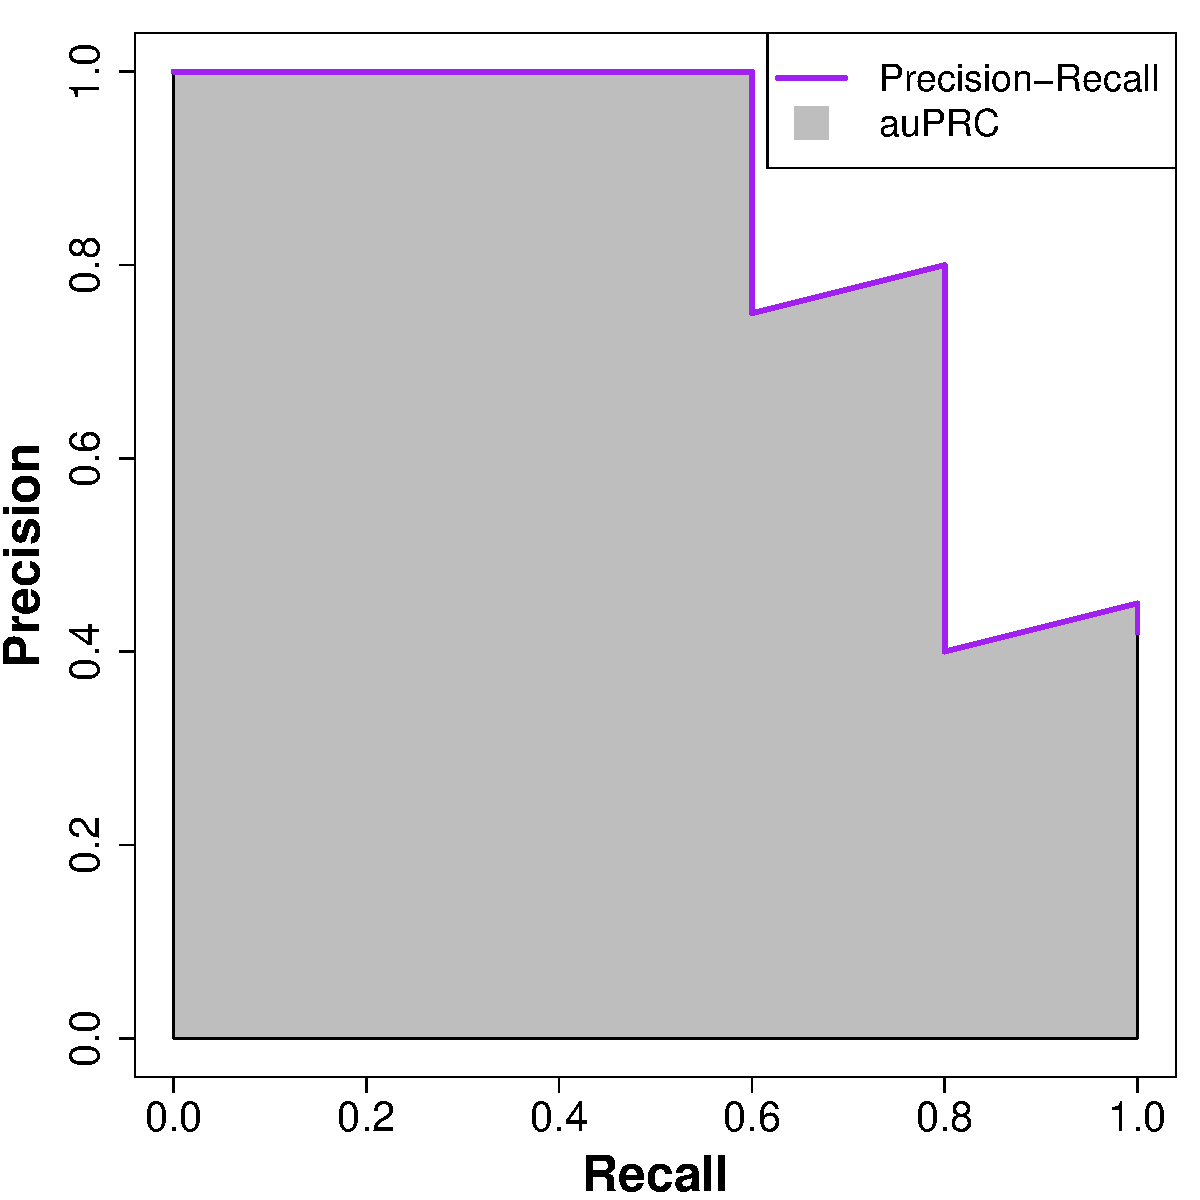
\includegraphics[scale=0.5]{precision-recall-curve.pdf}};

\draw [decorate,decoration={brace,amplitude=14pt,aspect=0.5,mirror},xshift=-4pt,yshift=0pt,line width=0.4mm,draw=black] (5.1,-4.4) -- (5.1,4.4) node [black,xshift=9pt] {\footnotesize};

\node[xscale=1.2,yscale=1.2] at (10.4,0.1) {$\text{auPRC} \approx 0.831$};
\end{tikzpicture}

\end{document}